\documentclass[acmtog]{acmart}
\usepackage{graphicx}
\usepackage{subfigure}
% Title portion
\title{Assignment 3 : Ray-based Rendering and Loop Subdivision} 
\author{Name:\quad Su'an Xia  \\ student number:\quad 18047482
	\\email:\quad xiasa@shanghaitech.edu.cn}

% Document starts
\begin{document}
\maketitle

\vspace*{2 ex}


\section{Introduction}
\subsection{Phong lighting model and shaders}
Requirement: A ray-based rendering program.
\\Main process: 
\\(1) Generating camera rays.
\\(2) Ray intersection test with a single triangle.
\\(3) Building a uniform grid for triangle meshes as the acceleration structure for ray-tracing.
\\(4) Ray intersection test with triangle meshes using uniform grid.
\\(5) Phong reflection model.

\vspace*{1 ex}
\subsection{Texture and shaders}
Requirement:A subdivision algorithm that smoothes meshes.
\\Main process:
\\(1) Subdivide closed surface;
\\(2) Subdivide non-closed surface;
\\\textbf{optional}:
\\(1) Reduce the time complexity to $o(p^{2}+f)$.
\\(2) Reduce the space complexity to $O(p^{2}+f)$.

\vspace*{2 ex}
\section{Implementation Details}
\subsection{Generating camera rays}
In camera.hpp, we only need to complete the Class 'Camera' and the function 'Ray generateRay(int dx, int dy)'.

\vspace*{1 ex}
\subsection{Ray intersection test with a single triangle}
In triangleMesh.hpp, we need to complete the function 'bool raySingleTriangleIntersection(Interaction\& interaction, const Ray\& ray, int v0\_idx, int v1\_idx, int v2\_idx)'
\\In this function, we need to calculate the value 't,v,w,n,e,d' following the formula. Then according the value of 'd' and some other limits, we choose to return false or true.
\vspace*{1 ex}
\subsection{Building a uniform grid}
In triangleMesh.hpp, we need to complete the function 'void buildUniformGrid()'
\\First we need to determine the appropriate dimensions of the grid by the formula.
\\Then we loop over each triangle's bounding box to see which grid will overlap with the triangle by calculation 'x * gridDim.y() * gridDim.z() + y * gridDim.z() + z'
\vspace*{1 ex}
\subsection{Ray intersection test}
In triangleMesh.hpp, we need to complete the function 'bool rayIntersection(Interaction\& interaction, const Ray\& ray) override'
\\The key idea is how we maintain the 'tMaxX tMaxY XtMaxZ' when we travers the light. Simply, we only update the smallest one by adding to the corresponding tDelta.
\\Also we need to pay atteneion to the situations where tMax is out the grid.
\\In each non-empty grid, we do the raySingleTriangleIntersection one by one.
\vspace*{1 ex}
\subsection{Phong reflection model}
In directLightingIntegrator.hpp, we need to complete the function 'Eigen::Vector3f radiance(Interaction* interaction, Ray * ray) override'
\\It is similat to what we did in assignment 2.
\subsection{build data struct}
In refine.hpp, we need to complete the function 'void ref::build\_data\_struct()'.
\\We keep 3 data,'P\_list L\_list F\_list'.
\\First we loop the 'out\_v\_index' to fullfill the P\_list.
\\Then wee loop the face to fullfill the L\_list. If one line is repeated, then it is not a border line.
\\Last we loop the L\_list to chech if it is a border line. If it is a border line, then we mark the corresponding points border.
\vspace*{1 ex}
\subsection{loop subdivision}
In refine.hpp, we need to complete the function 'void ref::loop\_subdivision()' and 'void subdivision(int division\_time)' in triangleMesh.hpp.
\\In additional to what we have, we need to keep 3 more data struct 'P\_new\_list L\_new\_list F\_new\_list'.
\\First we calculate the even points. It is easy by formula.
\\Then we calculate the odd points. It is also easy by formula.
\\Aftewards, we loop each face to complete the information of each new line and new face.
\\Last we loop the line to complete the 'border' information of certain points.
\\In the triangleMesh.hpp, what we should is to determine the division\_time and coduct the specific alogrithm by cycle.

\vspace*{2 ex}

\section{Results}

\begin{figure}[h]
\centering
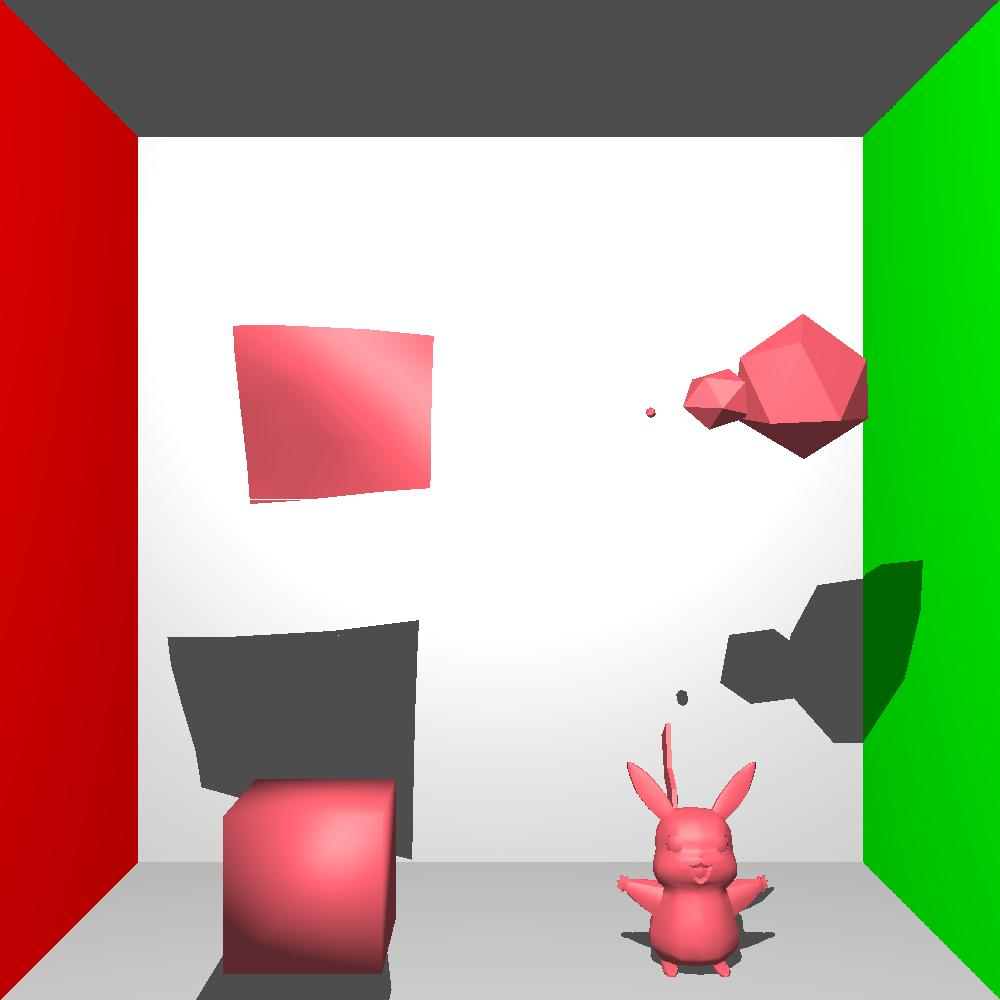
\includegraphics[width=6cm,height=8cm]{no-subdivision.jpg}
\caption{without loop subdivision}
\end{figure}

\begin{figure}[h]
\centering
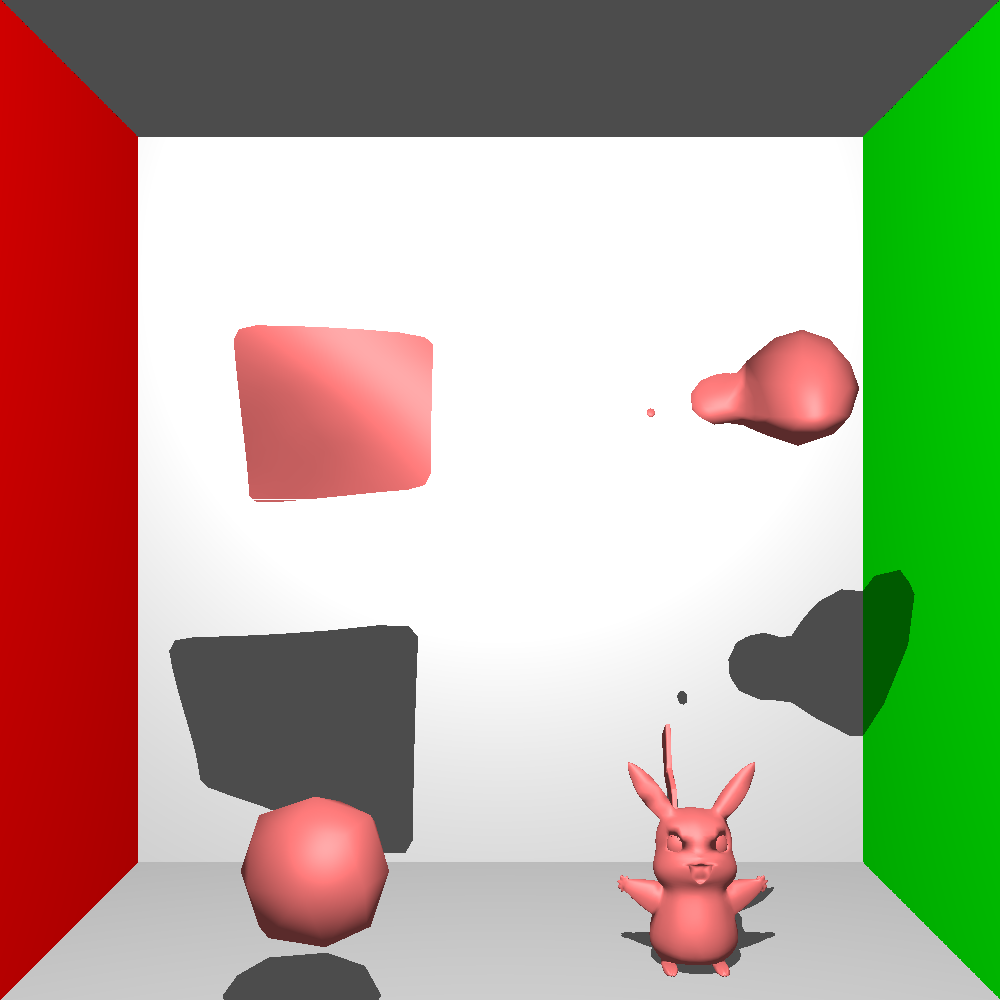
\includegraphics[width=6cm,height=8cm]{subdivision1.png}
\caption{division\_time = 1}
\end{figure}

\begin{figure}[h]
\centering
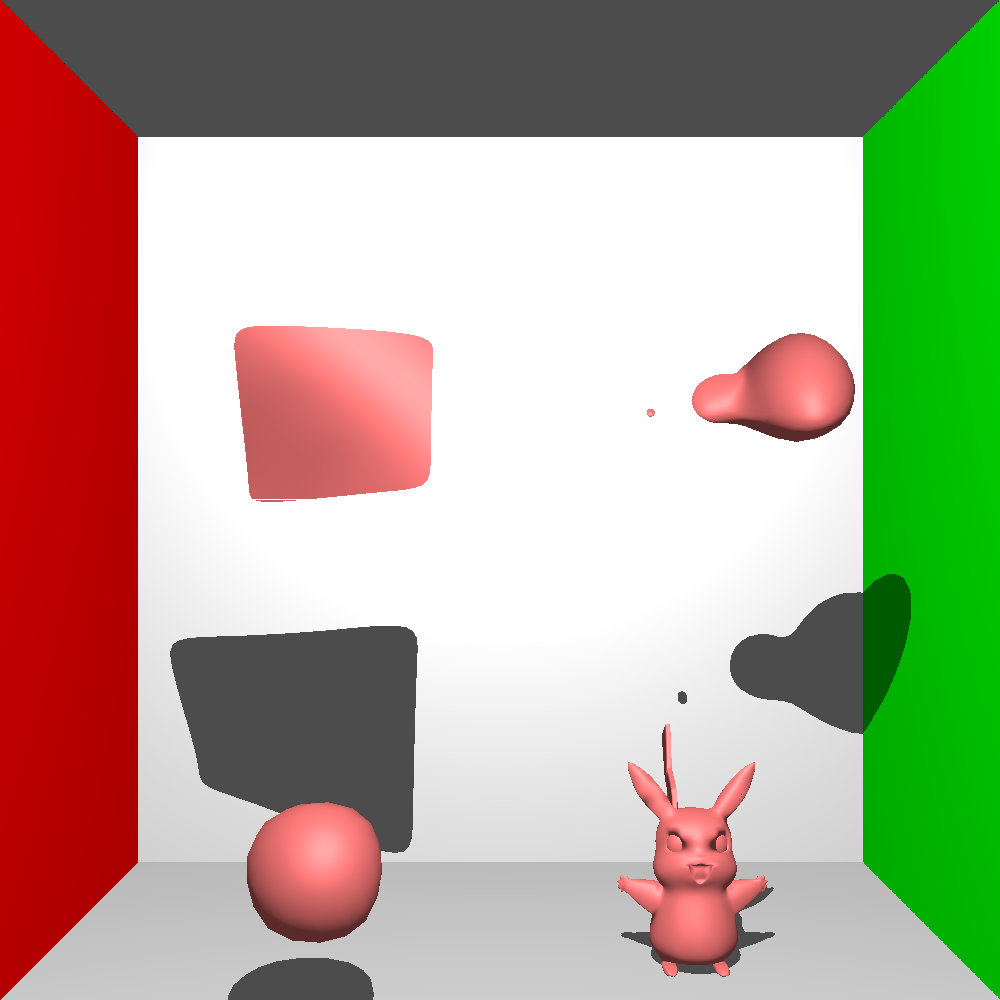
\includegraphics[width=6cm,height=8cm]{subdivision2.png}
\caption{division\_time = 2}
\end{figure}

\begin{figure}[h]
\centering
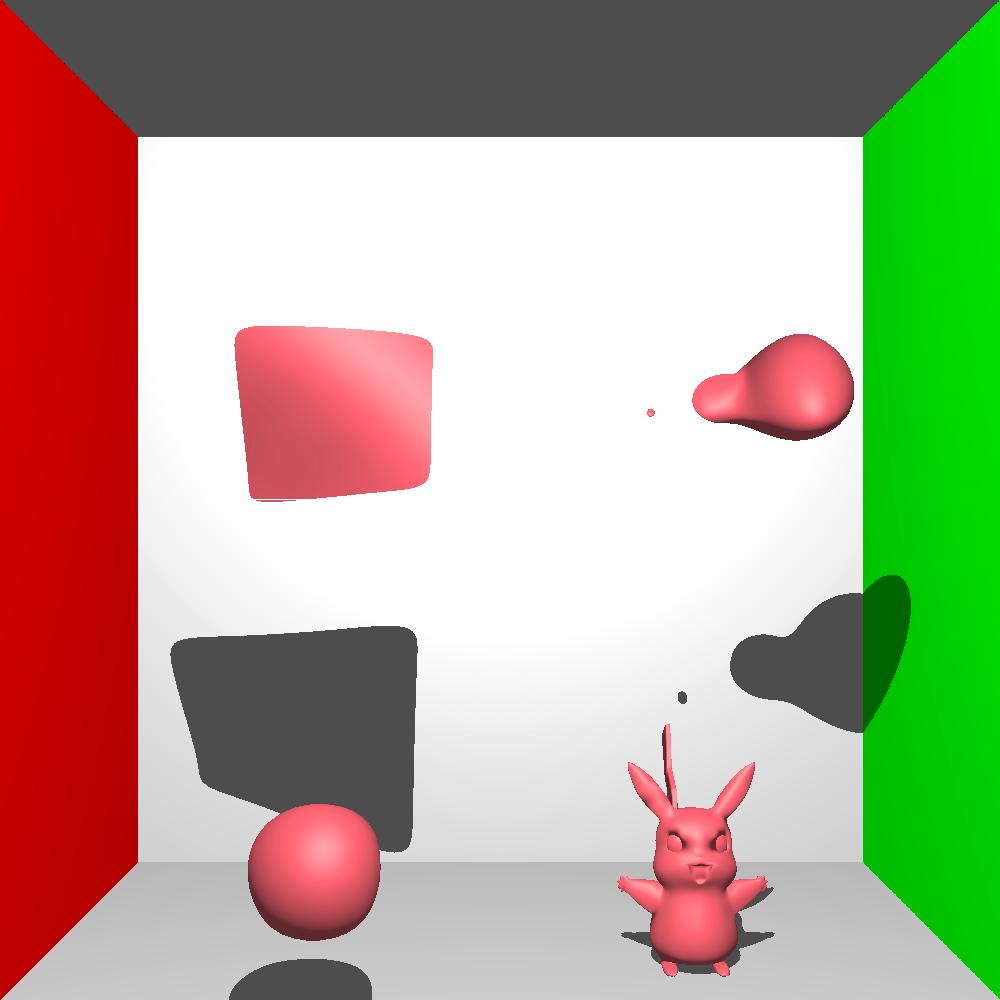
\includegraphics[width=6cm,height=8cm]{final.jpg}
\caption{division\_time = 3}
\end{figure}



\end{document}
